\chapter{Theoretical Background}
\label{chap:two}

\section{Credit Risk}

\subsection{Regulation}

\textbf{TBD}

\section{Terminology}
\begin{itemize}\setlength\itemsep{0em}
	\item \textbf{Target variable} - Dependent variable or response variable, which we want to predict or classify ($Y$). In this case we want to predict a defaut status (Yes or No).
	\item \textbf{Feature} - Predictor, independent variable or explanatory variable ($X$), which we want to use to predict the target variable $Y$.
	\item cross validation
	\item over fitting
\end{itemize}


\textbf{TBD}
\section{Algorithms}
\label{sec:algorithms}

In this section, several algorithms, which are used in the machine learning implementation, are going to be described. Since the goal is to predict whether or not given client will default, henceforth only (binary) classification algorithms as a part of the supervised learning are described. In other words, regression models and unsupervised learning algorithms are out of the scope of this thesis.
\subsection{Logistic Regression}

Despite the algorithm's name, it is actually not a regression but rather a classification model.
In contrast, a linear regression's target variable is continuous whereas regarding a logistic regression, the target variable is categorical (or rather dichotomous in case of binary classification) \citep{wendler2021data}.
For the probability estimation it is using a logistic, or so-called sigmoid function, which maps any real value within the range of 0 to 1 and takes a S-shaped curve as can be seen in \autoref{fig:sigmoid}.

\begin{figure}[H]
    \centering
    \caption{Logistic function}\vspace{0.5em}
    \label{fig:sigmoid}\
    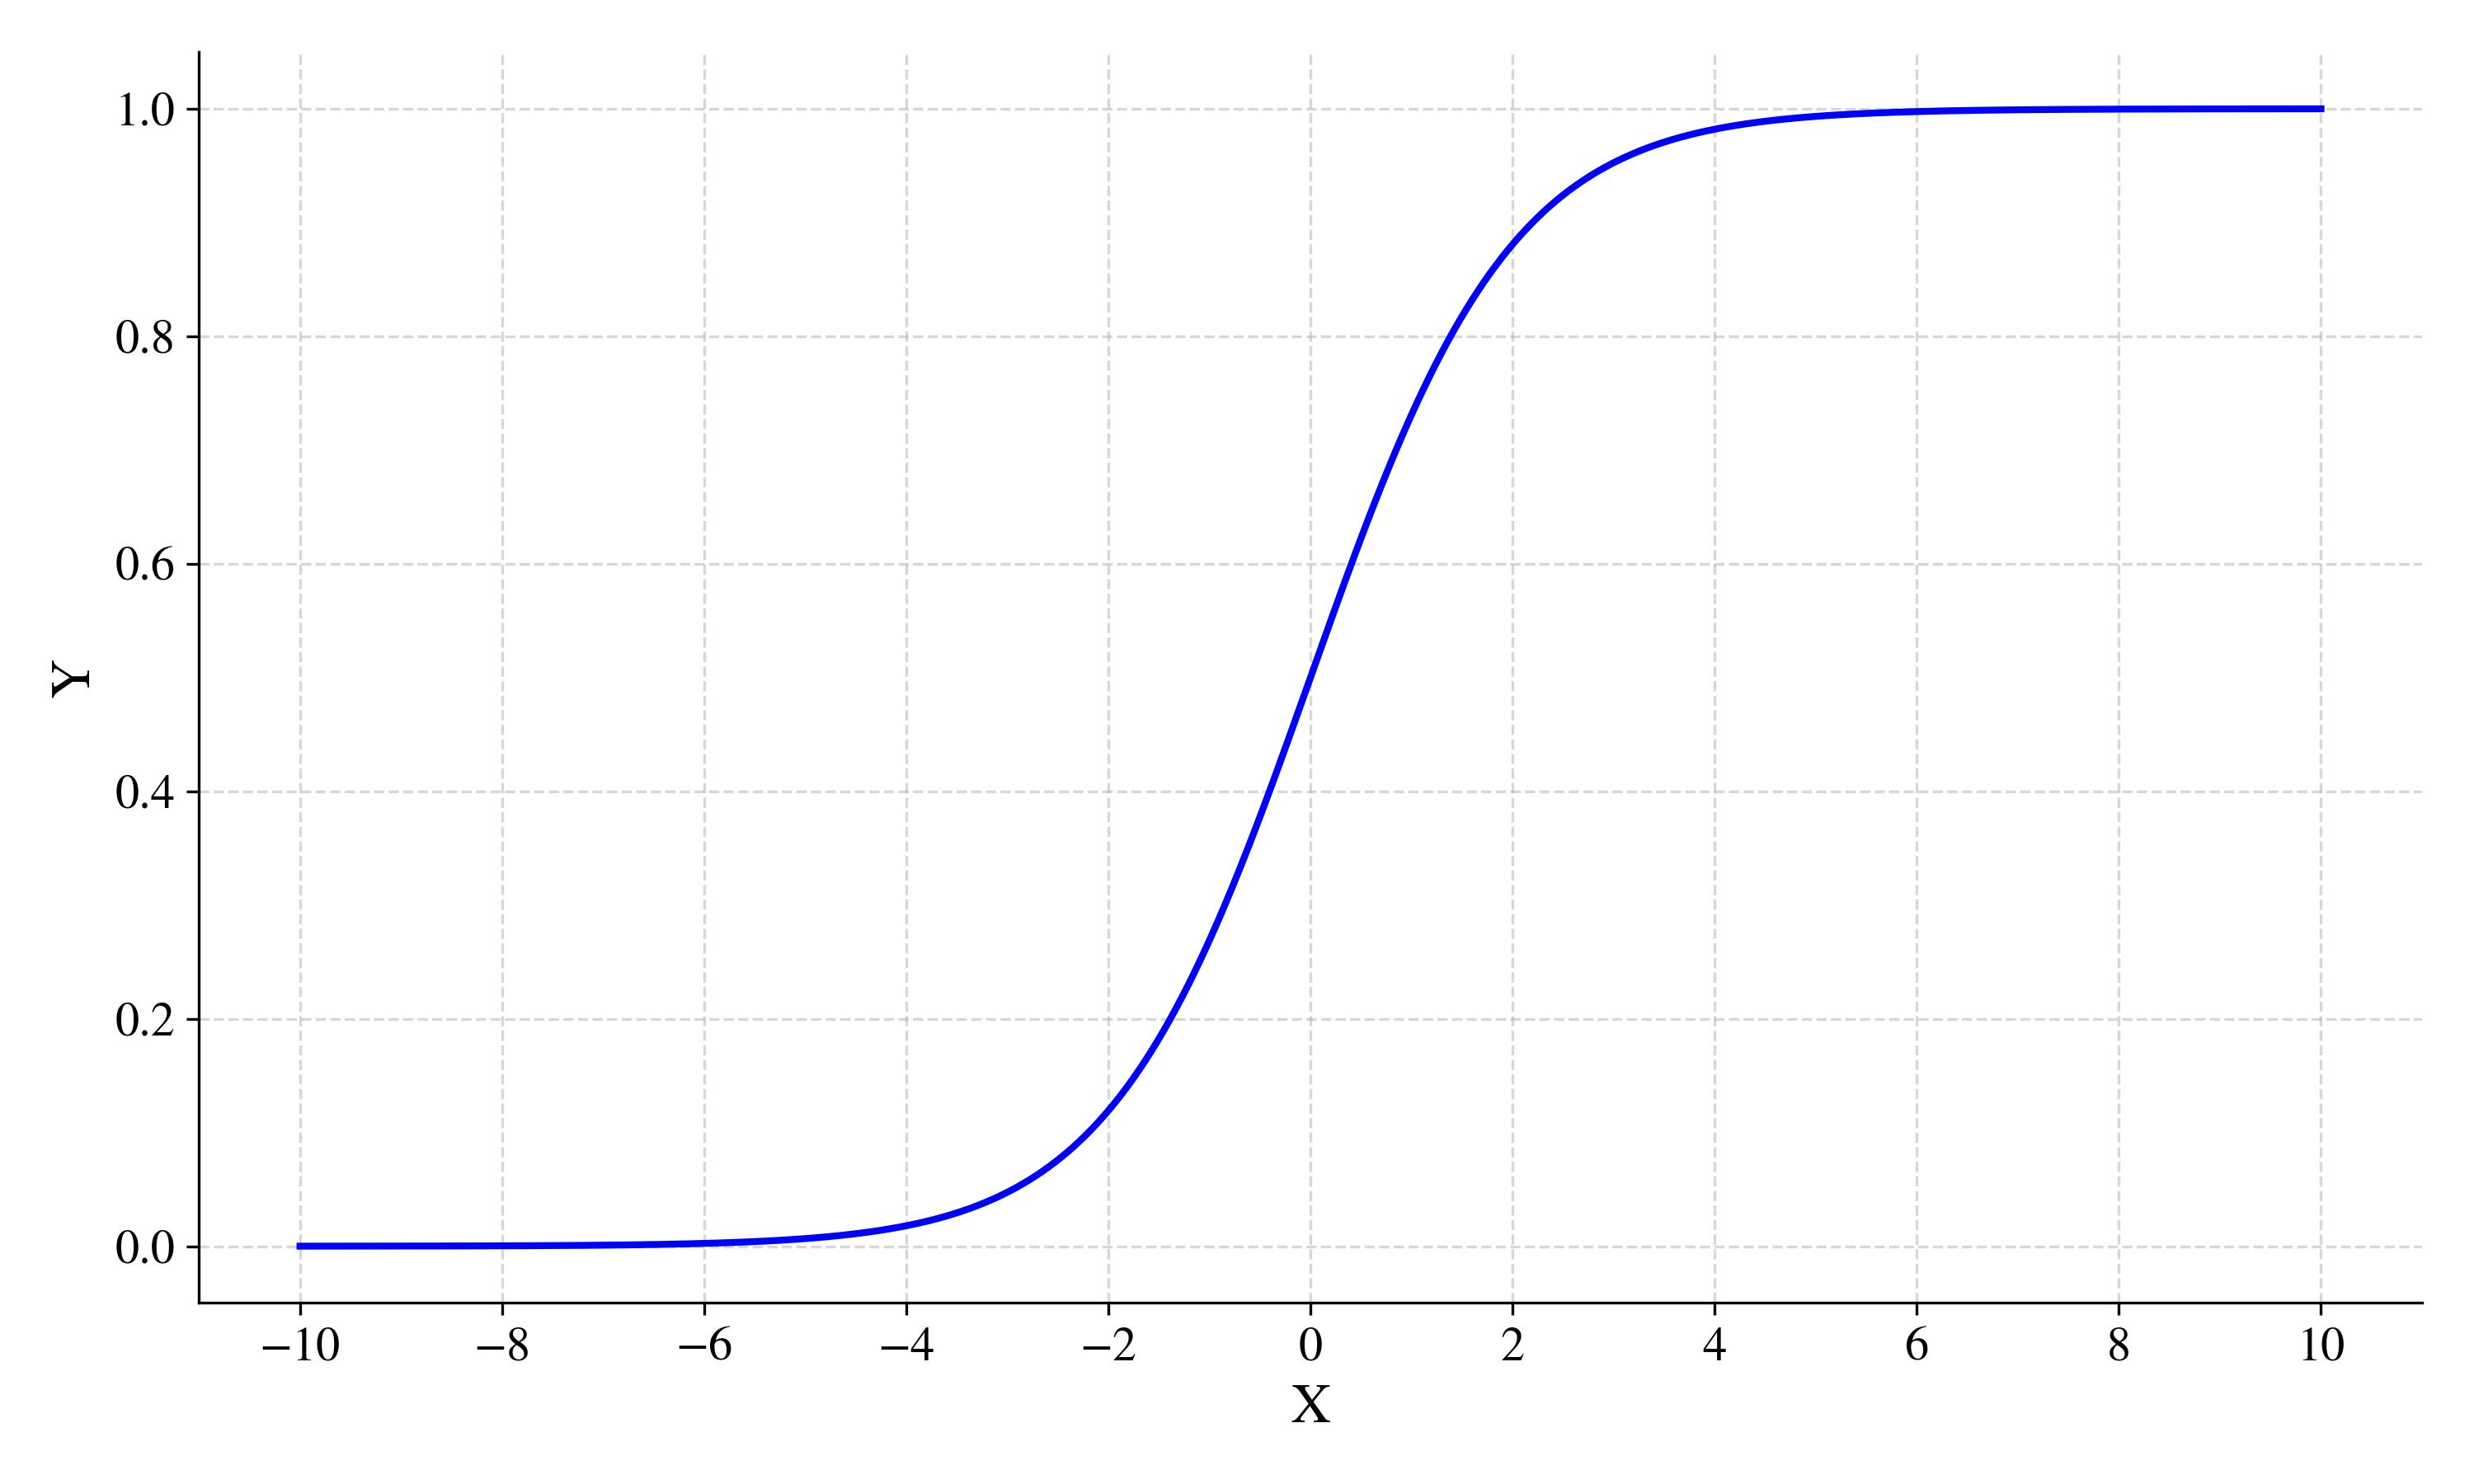
\includegraphics[width=130mm]{Figures/sigmoid.jpg}
    \centering{\begin{source}Author's simulation in Python\end{source}}\vspace{-1em}
\end{figure}

The linear form of the logistic regression with n features can be written as:

\begin{equation}\label{eq}
    \ln\left(\frac{P}{1-P}\right) = \beta_0  + \sum_{i=1}^{n} \beta_i X_i
\end{equation}

where $P$ is the probability of the occurred event, conditional on the set of given features. Let us denote $Y=1$ as an observed target instance where the event occurred (e.g., default), then:
\begin{equation}\label{eq}
    P = \operatorname{Pr}(Y=1 \mid X)
\end{equation}

Therefore, the term within the natural logarithm are the odds or more particularly, the ratio of the probability of the event with respect to the probability of non-event, both conditional on the same set of given features.
\begin{equation}\label{eq}
    \begin{aligned}
    \frac{P}{1-P}  {} & = \frac{\operatorname{Pr}(Y=1 \mid X_1,X_2,\ldots,X_n)}{1-\operatorname{Pr}(Y=1 \mid X_1,X_2,\ldots,X_n)} \\
    & = \frac{\operatorname{Pr}(Y=1 \mid X_1,X_2,\ldots,X_n)}{\operatorname{Pr}(Y=0 \mid X_1,X_2,\ldots,X_n)}
\end{aligned}
    \end{equation}

Referring to the previous equations, solving for $P$, henceforth we get a final equation for computing the probability of occurred event with usage of logistic regression:

\begin{equation}\label{eq}
P = \frac{1}{1+e^{-\left(\beta_0 + \displaystyle\sum_{i=1}^{n} \beta_i X_i\right)}}
\end{equation}

\subsection{Decision Tree}
\label{subsec:dt}

Decision tree (DT) is a rule--based algorithm which aims to partition the data into smaller and more homogeneous subsets. Such tree contains nodes, which are also visualized in \autoref{fig:dtnodes}, namely:
\begin{itemize}\setlength\itemsep{0em}
	\item Root node - the topmost node of the tree where the splitting begins.
	\item Internal node - the non--terminal nodes as a result of the split and can be further split into another subsets.
	\item Leaf node - the terminal nodes as a results of the split and cannot be further split into another subsets.
\end{itemize}
\begin{figure}[H]
    \centering
    \caption{Decision Tree's Nodes}\vspace{0.5em}
    \label{fig:dtnodes}\
    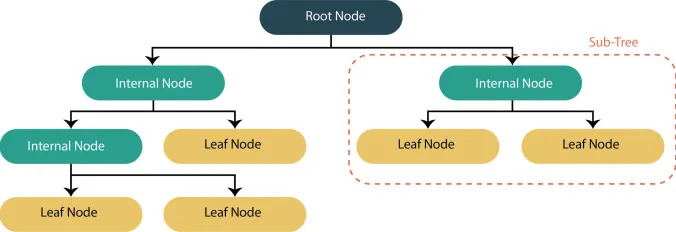
\includegraphics[width=130mm]{Figures/dtnodes.jpg}
    \centering{\begin{source}\citep{gauhar2020decision}\end{source}}\vspace{-1em}
\end{figure}

The splitting process is based on the homogeneity or so called purity of the node with respect to the target variable \citep{provost2013data}.
In other words, we want to have the node as pure as possible which means that the node should contain as high proportion of one class as possible.
In this case, the node should either contain high proportion of defaulters or non--defaulters, respectively.
Such splitting processs starts from the root node and continues until the leaf nodes are pure enough or until the stopping criteria are met.
The stopping criteria can be either a maximum depth of the tree, minimum number of observations within the node or minimum number of observations within the leaf node.
One way to measure impurity is using Entropy which ranges from 0 to 1 and is defined as:
\begin{equation}\label{eq}
    E = -\sum_{i=1}^{n} p_i \log_2 \left(p_i\right)
    \end{equation}
where $p_i$ is the probability of the occurrence of the event $i$, or in other words, it is a fraction of the observations belonging to the class $i$ within given node. In credit risk modelling terms, it is a proportion of defaulters within given node and $1-p_i$ is a proportion of non--defaulters within given sample.
The lower Entropy value, the purer the node is, i.e., the more homogeneous the subset is, where the frequency of one class is dominant to other class.
Therefore, the goal is to minimize the Entropy value since we want to have the purest nodes as possible, i.e., the nodes where is either a high proportion of defaulters or non--defaulters. 
However, the Entropy is not the only way to measure the impurity of the node. Another way is using Gini Impurity which ranges from 0 to 0.5 and is defined as:
\begin{equation}\label{eq}
    G = 1 - \sum_{i=1}^{n} p_{i}^{2}
\end{equation}
Both impurity measures are depicted in \autoref{fig:impurity} which we want to both of them minimize. Thus, we choose such feature and such rule which result in the lowest impurity measure. Such process is repeated until the stopping criteria are met or until the leaf nodes are pure enough.
\begin{figure}[H]
    \centering
    \caption{Gini Impurity vs. Entropy}\vspace{0.5em}
    \label{fig:impurity}\
    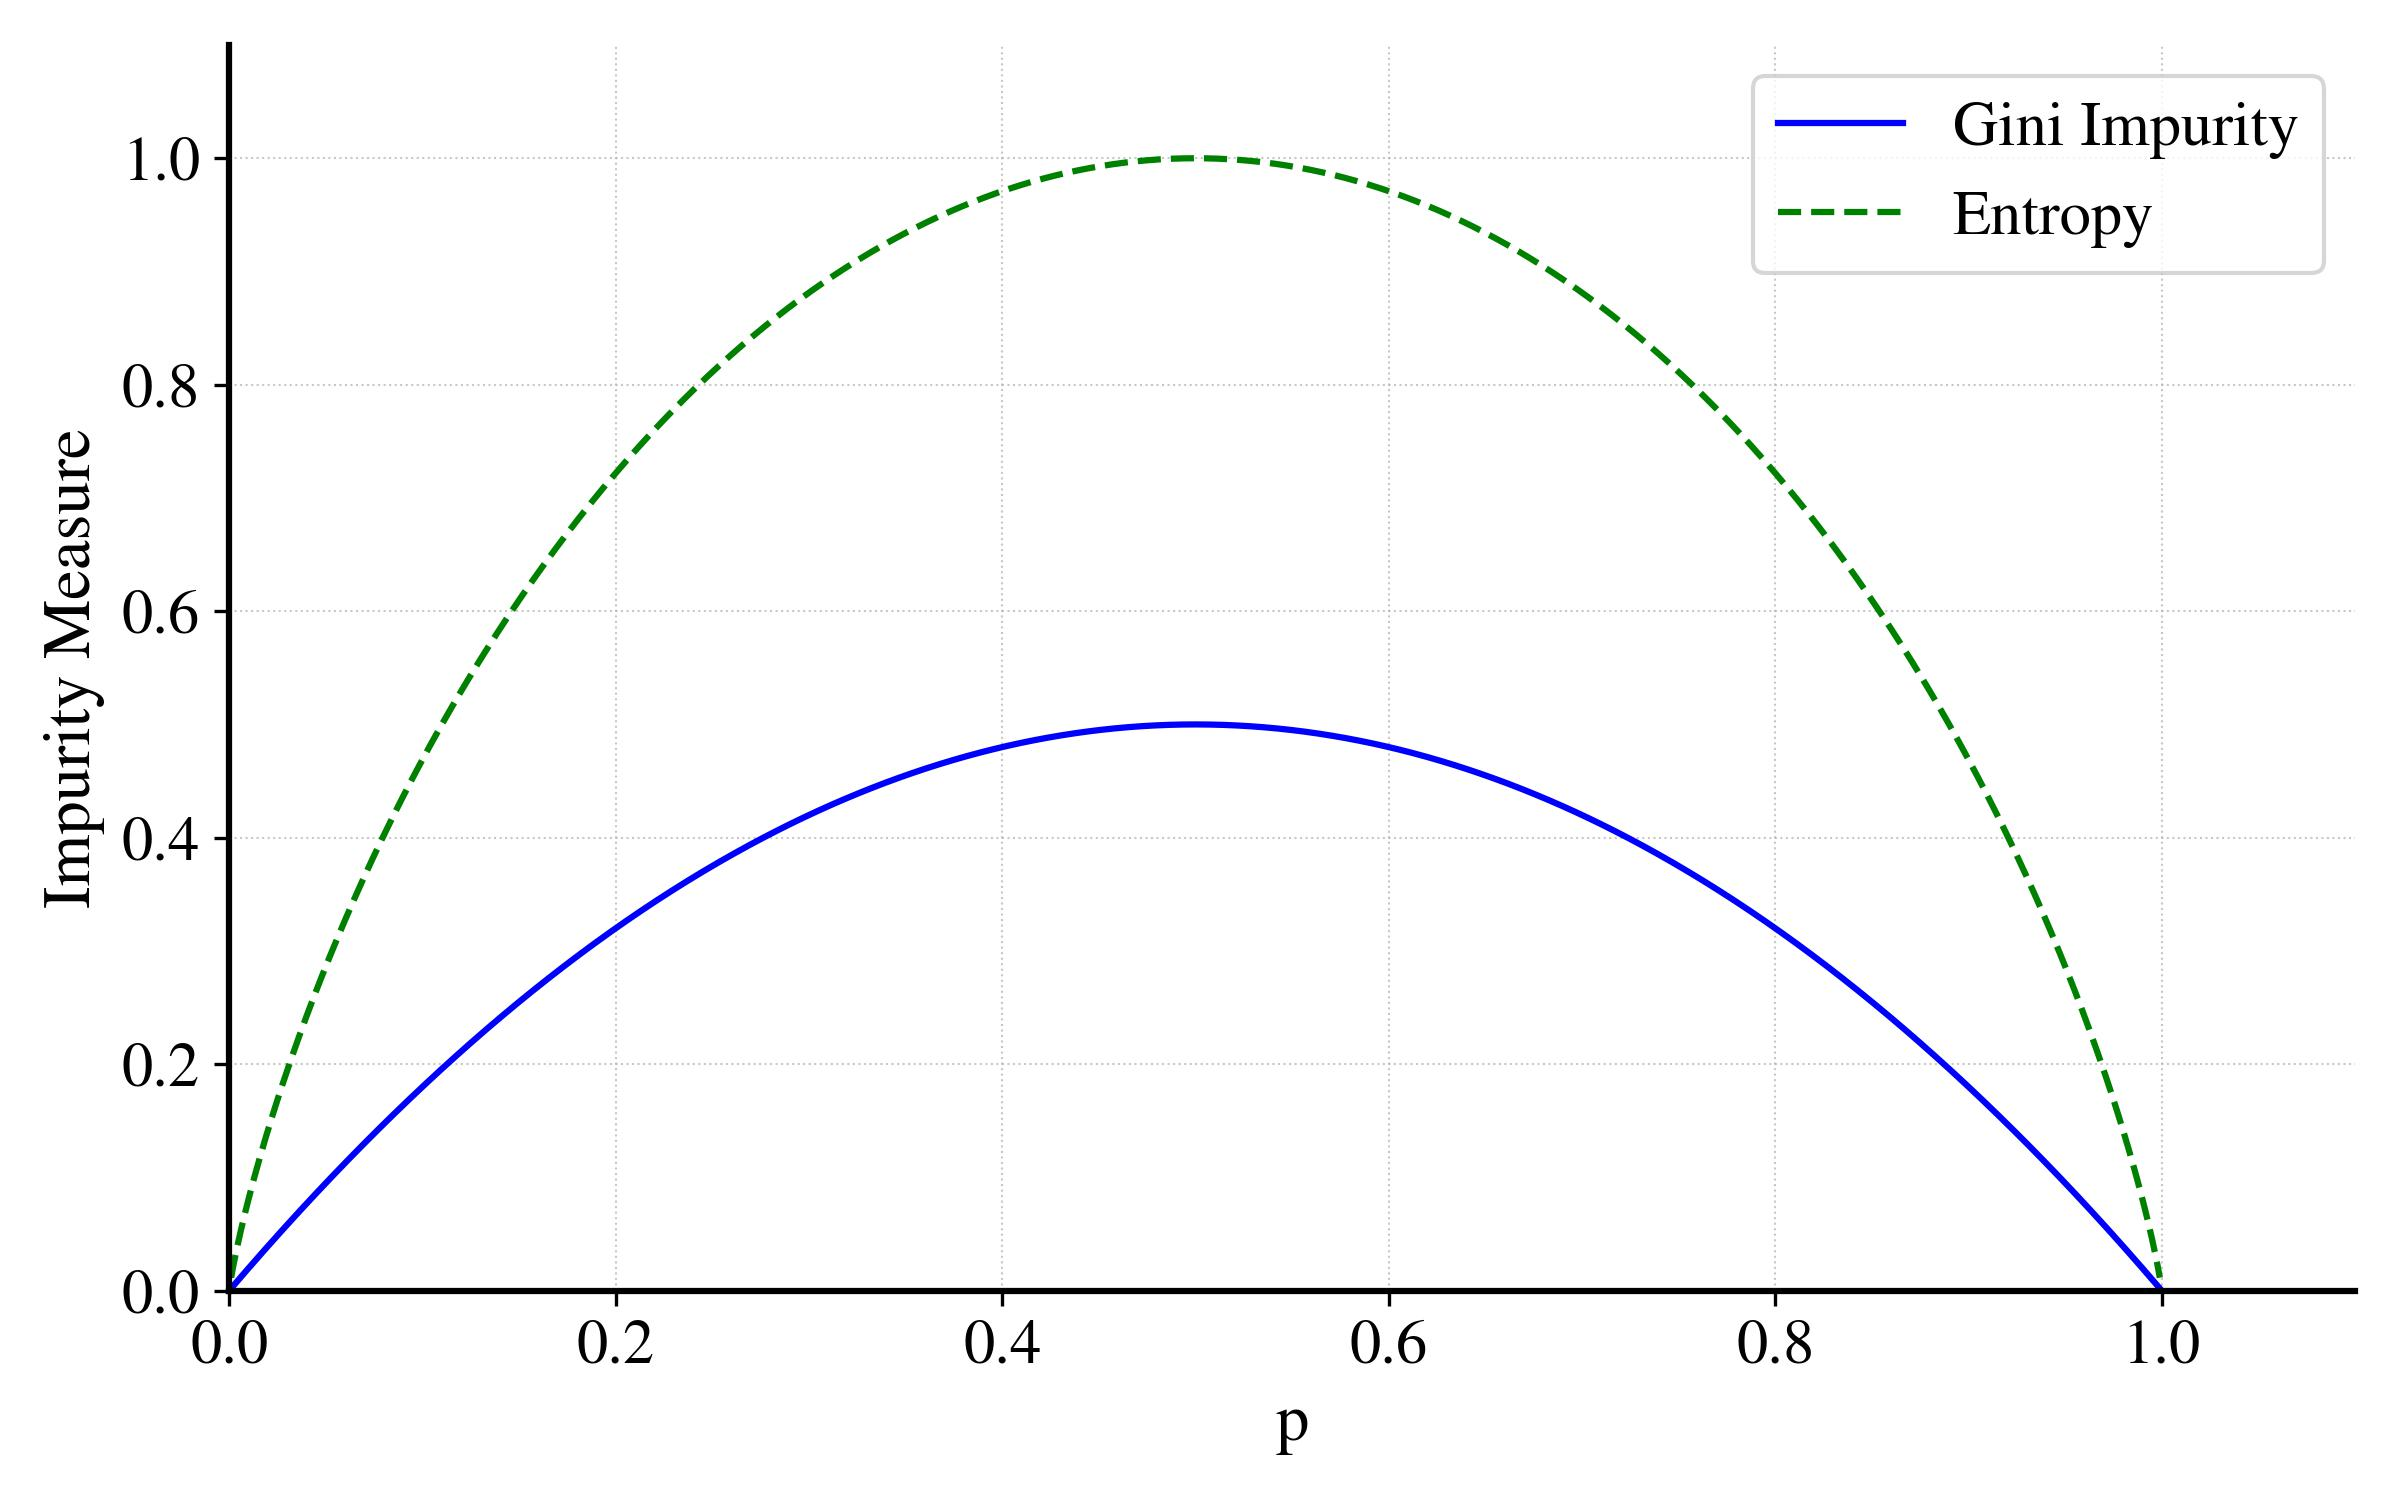
\includegraphics[width=130mm]{Figures/impurity.jpg}
    \centering{\begin{source}Author's simulation in Python\end{source}}\vspace{-1em}
\end{figure}

After the training, the DT predicts the target variable based on the rules which are stored in the tree.
The prediction process starts from the root node and continues until the leaf node is reached. Within the leaf node, the prediction can be either the most frequent class within the node or the probability of the occurrence of the event, i.e., the proportion of defaulters within given node.

\subsection{Naive Bayes}

Naive Bayes is a classification and probabilistic machine learning algorithm which is based on the Bayes theorem:

\begin{equation}\label{eq}
    \operatorname{Pr}\left(C=c \mid E \right) = \frac{\operatorname{Pr}\left(C=c\right) \times \operatorname{Pr}\left(E \mid C=c\right)}{\operatorname{Pr}\left(E\right)}
\end{equation}

where:
\begin{itemize}\setlength\itemsep{0em}
	\item $\operatorname{Pr}\left(C=c \mid E \right)$ is the posterior probability which is the probability that the target variable $C$ takes on the class of interest $c$ after taking the evidence $E$.
	\item $\operatorname{Pr}\left(C=c\right)$  is the prior probability of the class $c$ is the probability we would assign to the class $c$ before seeing any evidence $E$.
	\item $\operatorname{Pr}\left(E \mid C=c\right)$ is the probability of seeing the evidence $E$ conditional on the given class $c$.
	\item $\operatorname{Pr}\left(E\right)$ is the probability of the evidence $E$.
\end{itemize}

With regards to the binary classification, we can substitute $Y$ as a target variable instead $C$, and set of features $X$ which will refer to the set of evidence $E$., henceforth the probability of $Y$ using the Naive Bayes algorithm can be mathematically expressed as:

\begin{equation}\label{eq}
    \operatorname{Pr}\left(Y \mid X \right) = \frac{\operatorname{Pr}\left(Y\right) \times \operatorname{Pr}\left(X \mid Y \right)}{\operatorname{Pr}\left(X\right)}
\end{equation}

One of the assumptions of this algorithm is the conditional probabilistic independence among the features.
Since all the $X$ features' values combinations do not have to appear at all, we assume their independence \citep{cichosz2014data}.
Therefore, instead of computing the probability of all features together, conditional on the class event, for each feature $X$ we the conditional joint probability of $X$ given the class event. Hence:
\begin{equation}\label{eq}
    \operatorname{Pr}\left(X  \mid Y \right) = \prod_{i=1}^{n} \operatorname{Pr}\left(X_i \mid Y\right)
\end{equation}

Furthermore, the second adjustment is applied to the denominator of the Bayes theorem, i.e., $\operatorname{Pr}\left(X\right)$ - since such probability is constant over all the values of the class event, we can omit it from the equation. Therefore, the probability of the class event $Y$ can be expressed as:
\begin{equation}\label{eq}
    \operatorname{Pr}\left(Y \mid X \right) = \prod_{i=1}^{n} \operatorname{Pr}\left(X_i \mid Y\right) \times \operatorname{Pr}\left(Y\right)
\end{equation}

During the training process, the Naive Bayes algorithm computes $\operatorname{Pr}\left(Y\right)$ and $ \operatorname{Pr}\left(X \mid Y \right)$ for each class event $Y$ and each feature $X$.
In terms of default status, it calculates the proportion of defaulters  $\operatorname{Pr}\left(Y = 1\right)$ and non--defaulters $\operatorname{Pr}\left(Y=0\right)$ within given training sample as well as the proportion of defaulters and non--defaulters within given feature $X$.


When it comes to the predictions or classification of new instances, we use the trained Naive Bayes model, i.e., the computed probabilities $\operatorname{Pr}\left(Y\right)$ and $ \operatorname{Pr}\left(X \mid Y \right)$ for both default and non--default class.
Specifically, based on the new instance's features $X$, we determine the computed $\operatorname{Pr}\left(Y\right)$ and $ \operatorname{Pr}\left(X \mid Y \right)$ for both classes and aftewards, as a predicted class, we choose such class with the highest posterior probability. In general, the prediction while maximizing posterior probability is given as:
\begin{equation}\label{eq:nb-corrected}
    \operatorname{Pr}\left(Y \mid X \right) = \operatorname{argmax}_{y \in Y} \operatorname{Pr}\left(X \mid Y = y\right) \times \operatorname{Pr}(Y = y)
\end{equation}
Specifically, in terms of binary classification for prediction of given class, whether it is default or non--default, we can compute the probability of the default event ($1$) and non--default event ($0$) and choose the class with the higher probability.
\begin{equation}\label{eq}
    \operatorname{Pr}\left(Y \mid X \right)  = \max \left(\operatorname{Pr}\left(Y=1 \mid X\right), \operatorname{Pr}\left(Y=0 \mid X\right)\right)
\end{equation}
where:
\begin{equation}
    \operatorname{Pr}\left(Y=0 \mid X \right) = \operatorname{Pr}\left(Y=0\right) \times \prod_{i=1}^{n} \operatorname{Pr}\left(X_i \mid Y=0\right)
\end{equation}
respectively:
\begin{equation}
    \operatorname{Pr}\left(Y=1 \mid X \right) = \operatorname{Pr}\left(Y=1\right) \times \prod_{i=1}^{n} \operatorname{Pr}\left(X_i \mid Y=1\right)
\end{equation}
\subsection{K-Nearest Neighbors}

The goal of K-nearest Neighbors algorithm (also known as KNN) is to find $k$ instances that are most similar to particular instances y in the n-dimensional space, where n is the number of features.
The principle of this algorithm consists in the similarity between the instances as it assumes that the similar instances are close to each other.
Based on the predetermined $k$ neighbors, it will predict the class based on the k nearest instances.


There are several ways how to measure the distance. The most used one is the Euclidean distance. Geometrically, it is a straight line between the two points  and within two-dimensional space, it can be derived from the Pythagorean theorem, where the hypotenuse is the straight line measuring the distance. In the n-dimensional space, we take the sum the squared differences between the data points $x$ and $y$, underneath the square root in order to compute the total Euclidean distance.
\begin{equation}\label{eq}
d_{Euclidean}(x,y) = \sqrt{\sum\limits_{i=1}^{n} (x_i - y_i)^2}
\end{equation}

Other distance measure is the Manhattan distance measure, which is known as a city block distance, referring to the real-life problems, more particularly in order to reach particular destination, we have to take the path in between the blocks.
Mathematically, it is similar to the Euclidean distance, but instead of squared differences, it sums the absolute differences between the data points.
\begin{equation}\label{eq}
d_{Manhattan}(x,y) = \sqrt{\sum\limits_{i=1}^{n} |x_i - y_i|}
\end{equation}

The last measure is the Minkowski distance which is the generalized form Euclidean or Manhattan distance respectively.
It depends on p which represents the order of the norm. Hence, the Euclidean distance has the second order of the norm, whereas Manhattan distance has the first order of the norm.
\begin{equation}\label{eq}
d_{Minkowski}(x,y) = \sqrt[p]{\sum\limits_{i=1}^{n} |x_i - y_i|^p}
\end{equation}

Within the training process, KNN memorizes training instances and afterwards when it encounters a new instance, it tries to search for such training instance(s) which most strongly resembles the new instance \citep{witten2011data}.
Therefore, After the training process, when it comes to the prediction, the KNN compares the new instance to the training instances, calculates the distances between the the new input and the training instances, and predicts the class based on on the majority voting within the $k$ nearest neighbors, or predicts the probability scores as the fraction of positive instances within the $k$ nearest neighbors.


On the following \autoref{fig:knn-example}, let us consider 2--dimensional space and that $k$ is equal to 4, hence we are looking at four nearest neighbors for such new instance. Further, let us consider two classes - red squares and green triangles.
By looking at the four nearest neighbors, we can observe that three out of the nearest neighbors are the red triangles.
Therefore, when applying majority voting, KNN would predict such instance as a red triangle, or would predict a probability score of 0.75 for the red triangle.

\begin{figure}[H]
    \centering
    \caption{K-Nearest Neighbors with $k=4$}\vspace{0.5em}
    \label{fig:knn-example}\
    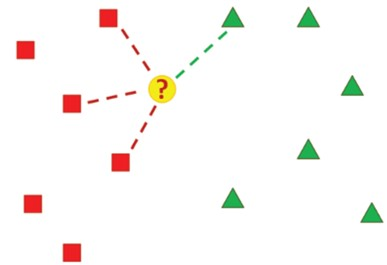
\includegraphics[width=80mm]{Figures/KNN_example.jpg}

    \centering{\begin{source}\citep{mucherino2009data}\end{source}}\vspace{-1em}
\end{figure}
\subsection{Random Forest}

Random forest is an ensemble algorithm which is a collection of decision trees where each tree is independently trained on on a bootstrap sample of the training data \citep{han2011data}, i.e., on a on a set which is randomly sampled from the training data with replacement which has the same size as the training data. In such way, each bootstrap sample is unique and can contain duplicates of the original data or does not have to contain all the original data.
Another aspect of randomness in such algorithm, particularly in the variability within trees, is the number of features considered for the split at each node.
Instead of considering all the features of the length $M$, it randomly selects a subset of features of the length $m$ (where $m<M$) and chooses the best split from the subset.
The training process of individual decision tree is the same as described in \autoref{subsec:dt}.

Within classifying new instances, the random forest algorithm predicts the class based on the majority voting of the individual decision trees or predicts a probability as an average of the probabilities of the individual decision trees \citep{randomforestmalley}, thus:
\begin{equation}
    \operatorname{Pr}\left(Y=1 \mid X \right) = \frac{1}{B} \sum_{b=1}^{B} \operatorname{Pr}\left(Y=1 \mid X, T_b \right)
\end{equation}
where $B$ is the number of trees and $T_b$ is the $b$-th tree.

\textbf{TBD}
\subsection{Gradient Boosting}

\textbf{TBD}
\subsection{Support Vector Machine}

\textbf{TBD}
\subsection{Neural Networks}

\textbf{TBD}

\section{Evaluation Metrics}

\textbf{TBD}

This section focuses on particular measures through which it is possible to determine a predictive power of model in terms of its performance.
The are many ways, how to evaluate the model's performance, therefore, only the most common ones and the most relevant are further described.
Note, since default prediction regards classification tasks, therefore regression's evaluation metrics are omitted.
If not stated otherwise, the higher metric measure, the better the model's performance is.
\subsection{Confusion Matrix and Derived Metrics}


Confusion matrix is a table which summarizes the classification model's performance with respect to the actual classes and predicted classes.
It is a square $n \times n$ matrix, where $n$ determines number of classes within the target variable.
Let us denote the confusion matrix as $C\left(f\right)$ for classification algorithm $f$. 
Its elements can be denoted as $c_{i,j}$ where $i$ and $j$ refer to the row and column indices, respectively, or more particularly, $i$ refers to the actual class and $j$ to the class predicted by the classifier $f$.
Each element of the confusion matrix refers to the number of instances corresponding to actual class $i$ and predicted class $j$ \citep{japkowicz2011evaluating}. For instance, the element $c_2,1$ would refer to the number of instances which have the actual class $2$ but have been classified as class $1$.
Mathematically, the confusion matrix can be written as following:

\begin{equation}\label{eq}
C = {c_{i,j} = \sum_{l=1}^{m}[(y_l=i) \land (f(x_l)=j)]}
\end{equation}

Or either in matrix form as:

\begin{equation}\label{eq}
    C_{i \times j} = \begin{bmatrix}
    c_{1,1} & c_{1,2} & \cdots & c_{1,j} \\
    c_{2,1} & c_{2,2} & \cdots & c_{2,j} \\
    \vdots & \vdots & \ddots & \vdots \\
    c_{i,1} & c_{i,2} & \cdots & c_{i,j} \\
    \end{bmatrix}
\end{equation}

From the given matrix, the diagonal elements represent the numbers of correctly classified instances, whereas the non-diagonal elements represent the numbers of misclassified instances.
Further, let us consider a binary classification - hence, the confusion matrix will have a form of $2\times 2$.

\begin{equation}
    C_{2 \times 2} = \begin{bmatrix}
    c_{1,1} & c_{1,2} \\
    c_{2,1} & c_{2,2} \\
    \end{bmatrix}
\end{equation}


We can this rewrite confusion matrix as:

\begin{equation}
    C_{2 \times 2} = \begin{bmatrix}
    TP & FN \\
    FP & TN \\
    \end{bmatrix}
\end{equation}

where:
\begin{itemize}\setlength\itemsep{0em}
    \item TP is the True Positive which refers to the number of instances which correspond to the actual class $True$ and indeed have been correctly classified as class $True$.
	\item $FP$ is the False Positive which refers to the number of instances which correspond to the actual class $True$, but have been incorrectly classified as class $False$. In the statistics and hypothesis--testing terms, it can be also called as Type 1 Error.
	\item $FN$ is the False Negative which refers to the number of instances which correspond to the actual class $False$, but have been incorrectly classified as class $True$. In the statistics and hypothesis--testing terms, it can be also called as Type 2 Error.
	\item $TN$ is the True Negative which refers to the number of instances which correspond to the actual class $False$ and indeed have been correctly classified as class $False$.
\end{itemize}

\subsubsection{Accuracy}
Such metric ranges from 0 to 1 and it describes in relatives terms how many instances the model has correctly predicted. Thus, the goal is to minimize the number of False Positives and False Negatives, or in credit risk modelling terms, number of defaulters which the model has classified as non--defaulters and number of non--defaulters which the model has classified as defaulters.
However, accuracy is inappropriate metric for evaluation when having imbalanced class, i.e., where the distribution of the target variable is skewed.
In such case, the model can achieve a relatively high accuracy even though it is not able to predict the minority class correctly \citep{brownlee2021failure}, thus it would lead to the misleading results.
This is the case of the credit risk modelling, when the loan portfolio oftenly have a lot of non--defaults and few defaults.
Therefore, it is deemed appropriate to consider other metrics when having imbalanced class.
\begin{equation}\label{eq}
    Accuracy = \frac{TP + FN}{TP + TN + FP + FN}
\end{equation}

\subsubsection{Recall}
Such metric is also known as True Positive Rate (TPR) or Sensitivity, which also ranges from 0 to 1, and it describes in relative terms how many actual \textit{True} instances the model has correctly predicted out of all the \textit{True} instances. Thus, the goal is to minimize the number of False Negatives, i.e., number of defaulters which the model has classified as non--defaulters.
A lower value of recall could therefore indicates that either the model is not able to predict correctly the $True$ classes resulting in low number of True Positives and/or high number of False Negatives.
Recall metris is useful when having imbalanced class and should be used instead of accuracy metric as it measures the model's ability to correctly identify instances of the minority class (i.e., defaults).
Mathematically based on the confusion matrix elements, it can be computed as:
\begin{equation}\label{eq}
    Recall = \frac{TP}{TP + FN}
\end{equation}

\subsubsection{Precision}
This metric describes in relative terms how many predicted \textit{True} instances are actually \textit{True}. Thus, the goal is to minimize the number of False Positives, i.e., number of non--defaulters which the model has classified as defaulters.
A lower value of precision could therefore indicates that either the model is not able to predict correctly the $True$ classes (low number of True Positives) or its prediction of $True$ classes is noisy (high number of False Positives).
Precision is another metric which should be used instead of accuracy when having imbalanced class as it tt measures the model's ability to correctly identify instances of the minority class while minimizing false positives (i.e., non--default instances which the model has classified as default).
Similarly, Precision also ranges from 0 to 1 and can be derived from the confusion matrix as follows:
\begin{equation}\label{eq}
    Precision = \frac{TP}{TP + FP}
\end{equation}
\subsubsection{F1 Score}
F1 score incorporates both Recall and Precision into a single value and takes on values between 0 and 1 as well.
Is it defined as a weighted harmonic mean of these two metrics \citep{brabec2020model} (where both Recall and Precision have uniform weights), and the goal is to minimize False Positives and False Negatives at the same time as within accuracy.
Nevertheless, F1 score is deemed as more appropriate metric when dealing with imbalanced class as it provides more balanced evaluation of model's performance in imbalanced datasets compared to accuracy.
\begin{equation}\label{eq}
    F1 = \frac{2 \times Precision \times Recall}{Precision + Recall} = \frac{2 \times TP}{2 \times TP + FP + FN}
\end{equation}

\subsubsection{Matthews Correlation Coefficient}
The drawback of Recall, Precision and F1 score is they are asymmetric measures, i.e., they do not take into account the True Negatives.
Therefore, such metrics' values will differ if we swap the positive and negative classes \citep{chicco2020advantages}, e.g., 1 would indicate non--default and vice versa.
In order to overcome such drawback, Matthews Correlation Coefficient can be used as it is symmetric and it takes into account all the four elements of the confusion matrix as well as it captures imbalanced class issue.
Methodologically, Matthews Correlation Coefficient is defined as a discretization of Pearson correlation for the case of binary variables \citep{boughorbel2017optimal}.
Pearson correlation coefficient is defined as:
\begin{equation}\label{eq}
    r(x,y) = \frac{\sum\limits_{i=1}^n (x_i - \bar{x})(y_i - \bar{y})}{\sqrt{\sum\limits_{i=1}^n (x_i - \bar{x})^2} \sqrt{\sum\limits_{i=1}^n (y_i - \bar{y})^2}}
\end{equation}
Thus, assuming that $x$ is the vector of True labels and $y$ is the vector of predictions, the Matthews Correlation Coefficient can be defined as:
\begin{equation}\label{eq}
    MCC = \frac{TP \times TN - FP \times FN}{\sqrt{(TP + FP) (TP + FN) (TN + FP) (TN + FN)}}
\end{equation}
Matthews correlation coefficient ranges from -1 to 1, where 1 indicates perfect model's predictions, -1 indicates that model misclassifies all the instances and 0 indicates that model's predictions are not better than random guessing.
\subsection{AUC}

In order to derive Area Under the Curve ($AUC$), first we need to define Receiver Operating Characteristics ($ROC$) curve.
ROC curve is two-dimensional visualization of the model performance as a probability curve in terms of True Positive Rate ($TPR$) and False Positive Rate ($FPR$) based on varying the given threshold.

Briefly, it can be construct as following: First, we need to sort the instances by the predicted probability and based on the given probability, we set a threshold - what will be above the threshold will be classified as $True$ instance and what is below the threshold will be classified as $False$ instance.
Based on these classified instances, the confusion matrix can be constructed and via which we can compute the $TPR$ and $FPR$ values.
Thus, if the probability is 1, the threshold will be 1 as well and hence:
\begin{itemize}\setlength\itemsep{0em}
    \item $TPR$ will be 0 because there is no probability which is higher than 1 and hence, everything will be classified as $False$ which will result into $TP$ of 0, and subsequently into $TPR$ of 0 as well.
	\item $FPR$ will be 0, too – since everything will be classified as $False$, therefore $FP$ will be 0 which implies $FPR$ to be 0, too.
\end{itemize}
On the other hand, if the probability is 0, the threshold will be 0 as well and hence:
\begin{itemize}\setlength\itemsep{0em}
    \item $TPR$ will be 1 because there is no probability which is lower than 0 and hence, everything will be classified as $True$ which will result into $FN$ of 0, and subsequently into $TPR$ of 1.
	\item $FPR$ will be 1, too – since everything will be classified as $True$, therefore $TN$ will be 0 which implies $FPR$ to be 1.
\end{itemize}

Thus, based on each threshold, the $TPR$ and $FPR$ will be to coordinates for single point within the graph and based on such points, we can construct the ROC curve.
Such visualization on the following \autoref{fig:roccurvetheory}.
Note the diagonal line represents a random model which randomly and correctly predicts the $True$ and $False$ classes in such way, that $FPR$ and $TPR$ are the same.
Logically, a decent model should perform better than the random model, thus it the ROC curve should be above the diagonal line.
Intuitively, the best possible theoretical model would have $TPR$ of 1 and $FPR$ of 0, meaning that all the $True$ actual classes should be predicted as $True$ and all the $False$ actual classes should not be classified as $True$
 Within the ROC curve, the given curve reaches the left top corner which corresponds to the coordinates of $TPR$ and $FPR$.

 \begin{figure}[H]
    \centering
    \caption{ROC Curve}\vspace{0.5em}
    \label{fig:roccurvetheory}\
    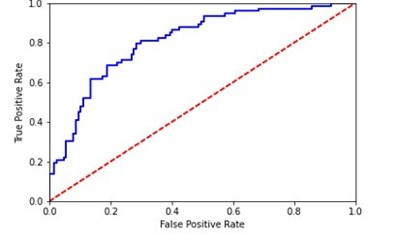
\includegraphics[width=100mm]{Figures/ROC_theory.jpg}

    \centering{\begin{source}Author's results in Python.\end{source}}\vspace{-1em}
\end{figure}

$AUC$ is basically the representation of ROC curve as a single number as it aggregates the performance on all possible thresholds.
$AUC$ can be interpreted as the probability that the randomly chosen actual $True$ instance is ranked higher than the randomly chosen actual $False$ instance.
Since ROC curve is a probability curve, thus it is considering distribution curve of $TP$ and distribution class of $TN$, separated by particular threshold – hence, $TP$ would have probability scores above the given thresholds, whereas $TN$ would have probability scores below the threshold.
If these curves do not overlap, meaning the model can perfectly distinguish between the $True$ and $False$ values, therefore the $AUC$ would be 1 and the ROC curve would reach the left top corner.
However, this idealistic situation does not occur in the practice at all, but rather the two distributions are overlapping since the misclassification of the classes takes the place.
The bigger overlap, the lower $AUC$ is.
If the distributions are completely overlapping, it implies the $AUC$ of 0.5, meaning that the model cannot distinguish between the $True$ and $False$ classes, which is the worst scenario.
On the other hand, if the distributions are totally opposite (meaning that the $TP$ instances would have probability scores below the given threshold, whereas the $TN$ instances would have probability scores above the given threshold), the $AUC$ would be 0 since the model is predicting the $True$ actual classes instead of $False$ and vice versa.

As the $AUC$ is an area present underneath the ROC curve, mathematically, it can be computed with the definite integral where $x$ is the given threshold:

\begin{equation}\label{eq}
    AUC = \int_{0}^{1} TPR \left(FPR^{-1}\left(x \right)\right) dx
\end{equation}

\subsection{Kolmogorov-Smirnov}

The Kolmogorov-Smirnov (KS) is non--parametric metric for assessing discriminant power of a model as it measures distance between the cumulative distribution functions (CDF) between two classes, and is quantified as a maximum vertical absolute difference between such two CDF's \citep{adeodato2016equivalence}.
In credit risk modelling terms, we can express KS as follows:
\begin{equation}\label{eq}
    \text{Kolmogorov Smirnov} = \max_{0 \le j \le 1} \left| F_D \left(j \right) - F_{ND} \left(j \right) \right|
\end{equation}
where $F_D$ and $F_{ND}$ are the cumulative distribution functions of default and non-default cases, respectively, and $j$ is the probability score threshold which ranges between 0 and 1.
\subsection{Somer's D}

The Somers' D is a metric which is part of the Kendall family of ranking measures. Particularly, assuming X-Y pairs, a Kendall's $\tau_{a}$ is defined as:
\begin{equation}\label{eq}
    \tau\left(X,Y\right) = \text{E} \left[ \text{sign}(X_i - X_j) \text{sign} (Y_i - Y_j) \right]
\end{equation}
Equivalently, Kendall's $\tau_{a}$ can be defined as the difference between the probability that the two X-Y pairs are \textit{concordant} and the probability that they are \textit{discordant}. X-Y pair is concordant if the larger of the $X$ values is paired with with larger of the $Y$ values, i.e, $X_i < X_j$ and $Y_i < Y_j$.
In contrast, X-Y pair is discordant if the larger of $X$ values is associated with smaller of $Y$ values or vice versa, i.e, $X_i < X_j$ and $Y_i > Y_j$, or $X_i > X_j$ and $Y_i < Y_j$ \citep{newson2002parameters}.
Therefore, Somers' D can be defined as the difference between the two conditional probabilities of concordance and discordance, given that the two $X$ values are unequal \citep{newson2014interpretation} as follows:
\begin{equation}
    D\left(Y \mid X\right) = \frac{\tau\left(X,Y\right)}{\tau\left(X,X\right)}
\end{equation}
In case of a binary classification, $X$ values would represent \textit{True} labels and $Y$ values would represent predicted probability scores as rank vectors. Such metric ranges from -1 to +1 (likewise as Matthews correlation coefficient +1). Thus, the higher value of Somers' D, the model's better ability to distinguish between borrowers who are likely to default and those who are not.

\subsection{Brier Score Loss}
Methodologically, Brier Score Loss is calculated in the same way as Mean Squared Error (MSE). However, Brier Score Loss is applied to the predicted probabilities (i.e., assumes that the target variable is dichotomous) \citep{comotto2022evaluation}, whereas MSE is rather used in regression tasks where is no assumption regarding the continuous target variable.
Henceforth, Brier Score Loss is defined as a mean squared error between the $True$ labels ($y$) and the predicted probabilities ($\hat{y}$) as follows:
\begin{equation}\label{eq}
    \text{Brier Score Loss} = \frac{1}{n} \sum_{i=1}^{n} (y_i - \hat{y}_i)^2
\end{equation}
Brier Score Loss ranges from 0 to 1, where the the ideal scenario would be Brier Score Loss of 0 - in such case, the model would be perfect predictive power.
\subsection{Jaccard Score}
Jaccard Score which is also known as Jaccard Index is a similarity metric as it measures similarity between the\textit{True} labels and predicted classes (0 or 1).
Let us denote $y$ as a vector of \textit{True} labels and $\hat{y}$ as a vector of predicted classes.
Hence, we can define Jaccard Score as the ratio of the size of intersection of $y$ and $\hat{y}$ to the size of union of $y$ and $\hat{y}$ \citep{leskovec2020mining}. Thus:
\begin{equation}\label{eq}
    \text{Jaccard Score} = \frac{|y \cap \hat{y} |}{|y \cup \hat{y} |}
\end{equation}
Likewise, Jaccard score ranges from 0 to 1 where the higher value indicates the higher similarity between the \textit{True} labels and predicted classes, hence the better model's performance.


\subsection{Log Loss}

Log loss, also know as logistic loss or cross--entropy loss, is a loss function metric which takes \textit{True} labels and predicted probabilities as an input and the minimize the difference between these two in a logarithmic function's form. Particularly, it indicates how close the predicted probabilities are to the corresponding $True$ labels. The more predicted probabilities diverges from the actual value, the more the log loss function penalizes the model's performance \citep{dembla2020intuition}.
\begin{equation}\label{eq}
    \text{Log Loss}  = -\frac{1}{N} \sum_{i=1}^{N} y_i \ln(p_i) + (1-y_i)\ln(1-p_i)
\end{equation}


Logically, the lower Log loss value, the better performance of the model is. As depicted in \autoref{fig:logloss}, we can observe the closer the predicted probability is closer to 1 with respect to the $True$ label being equal to 1, the more is the log loss function closer to 0 which is desired in terms of model's performance.
\begin{figure}[H]
    \centering
    \caption{Log Loss Function when $Y=1$}\vspace{0.5em}
    \label{fig:logloss}\
    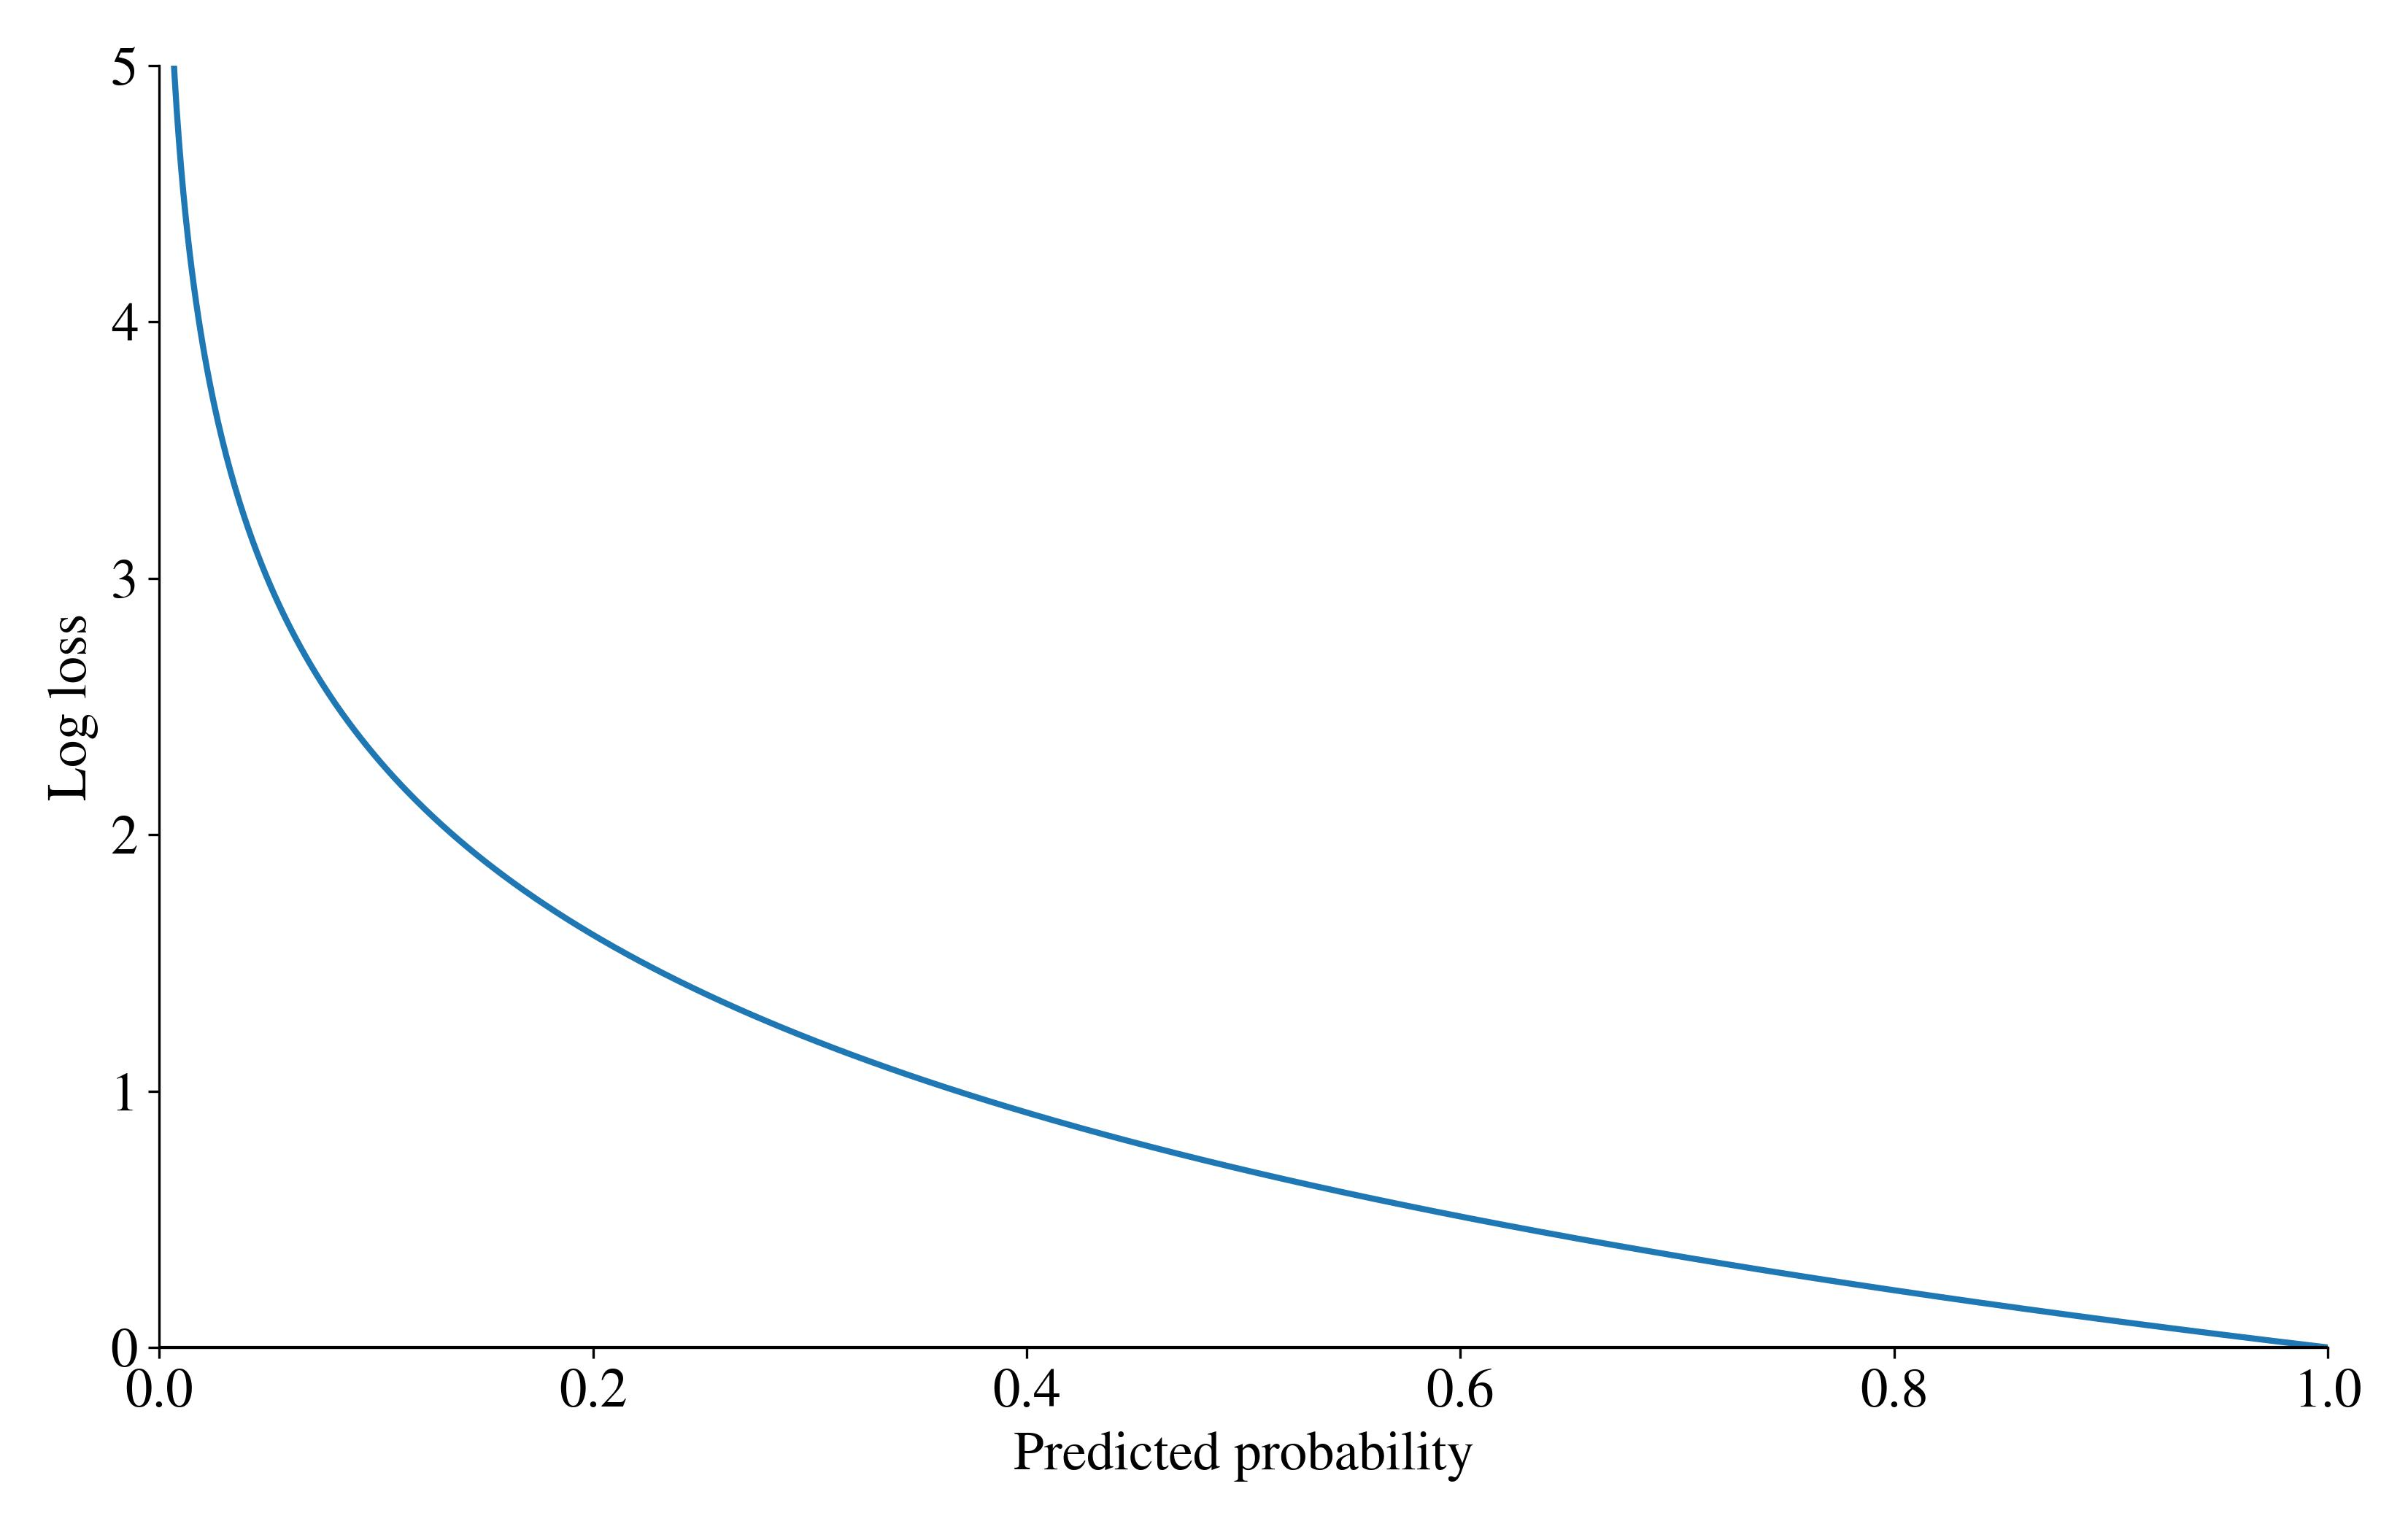
\includegraphics[width=130mm]{Figures/logloss.jpg}
    \centering{\begin{source}Author's simulation in Python\end{source}}\vspace{-1em}
\end{figure}